\section{Ứng dụng}
\label{sec:app}

\subsection{Yêu cầu}
Hệ thống có ba nhóm người dùng: Quản trị (ADMIN), Lễ tân (RECEPTIONIST) và Bác sĩ (DOCTOR). Đề yêu cầu $2 \times 2 = 4$ chức năng (không tính đăng nhập/đăng xuất); nhóm thực hiện 9 chức năng (Bảng~\ref{tab:fr}). Ma trận đủ 8 loại truy vấn ở Mục~\ref{sec:query-matrix}.

\begin{table}[H]
\centering
\caption{Danh sách chức năng}
\label{tab:fr}
\begin{tabularx}{\linewidth}{|c|X|c|p{4.6cm}|}
\hline
\textbf{FR} & \textbf{Chức năng} & \textbf{DBMS} & \textbf{Loại query chính} \\ \hline
FR1 & Quản lý hồ sơ bệnh nhân & SQL Server & a, b, c, d \\ \hline
FR2 & Quản lý bác sĩ \& khoa phòng & SQL Server & a, b, c, g \\ \hline
FR3 & Đặt lịch \& quản lý lịch hẹn & SQL Server & a, b, c, e, f + transaction + khoá \\ \hline
FR4 & Khám bệnh, kê đơn, hoá đơn & SQL Server & a, c + transaction nhiều bảng \\ \hline
FR5 & Tìm kiếm bệnh nhân đa điều kiện & SQL Server & e \\ \hline
FR6 & Chi tiết lượt khám & SQL Server & f (10 bảng) \\ \hline
FR7 & Thống kê & SQL Server & h \\ \hline
FR8 & Truy vấn nâng cao & SQL Server & g \\ \hline
FR9 & Theo dõi sinh hiệu real-time & \textbf{Cassandra} & a, d \\ \hline
(phụ) & Nhật ký truy cập & \textbf{Cassandra} & a, d \\ \hline
\end{tabularx}
\end{table}

\subsection{Kiến trúc và công nghệ}

\begin{figure}[H]
\centering
\begin{tikzpicture}[
    box/.style={draw, rounded corners, align=center, minimum height=1.1cm, text width=3.6cm, fill=blue!5},
    db/.style={draw, cylinder, shape border rotate=90, aspect=0.25, align=center, minimum height=1.4cm, text width=2.6cm, fill=orange!10},
    arr/.style={->, >=stealth, thick}]
  \node[box] (web) {\textbf{Trình duyệt}\\React 19 + Ant Design 6\\(Vite)};
  \node[box, right=1.6cm of web, text width=4.4cm] (api) {\textbf{Node.js 24 / Express 5}\\routes $\rightarrow$ service $\rightarrow$ repository};
  \node[db, below left=1.2cm and -1.4cm of api] (mssql) {SQL Server 2022};
  \node[db, below right=1.2cm and -1.4cm of api] (cas) {Cassandra 5.0};
  \draw[arr] (web) -- node[above, font=\small]{HTTP/JSON, SSE} (api);
  \draw[arr] (api) -- node[left, font=\small]{mssql} (mssql);
  \draw[arr] (api) -- node[right, font=\small]{cassandra-driver} (cas);
\end{tikzpicture}
\caption{Kiến trúc n-tier của ứng dụng}
\label{fig:arch}
\end{figure}

\begin{itemize}
    \item \textbf{N-tier, phân lớp rõ ràng:} \textit{routes} (HTTP, validate bằng zod, phân quyền) $\rightarrow$ \textit{service} (nghiệp vụ, transaction) $\rightarrow$ \textit{repository} (duy nhất nơi viết SQL/CQL, luôn dùng tham số).
    \item \textbf{Polyglot persistence:} dữ liệu quan hệ và giao dịch trên SQL Server; dữ liệu ghi liên tục, đọc theo mẫu cố định trên Cassandra. Hai DB liên kết qua \texttt{patient\_id}/\texttt{user\_id}. Cách chia dựa trên kết luận của Mục~\ref{sec:demo}.
    \item \textbf{Bảo mật:} JWT, mật khẩu băm bcrypt, phân quyền theo vai trò ở cả API lẫn giao diện; token SSE không bị ghi vào log.
    \item \textbf{Môi trường:} Docker Compose (SQL Server + 1 hoặc 3 node Cassandra); \texttt{npm run db:init} tạo lại DB giống hệt nhau trên mọi máy.
    \item \textbf{Kiểm thử:} 14 test API end-to-end (\texttt{node:test}); kiểm thử giao diện bằng trình duyệt headless trên 9 luồng nghiệp vụ.
\end{itemize}

\subsection{Thiết kế dữ liệu}
\todo{Dương}{ERD SQL Server và mô hình Cassandra thiết kế theo truy vấn (Q1--Q4); nguồn: \texttt{docs/design/erd.md}.}

\subsection{Hiện thực và giao diện}

\subsubsection{FR3: Đặt lịch hẹn}
Lễ tân chọn bệnh nhân $\rightarrow$ bác sĩ $\rightarrow$ ngày, hệ thống hiện \textbf{lưới khung giờ trống} (Hình~\ref{fig:fr3-booking}). Giờ đã đặt hoặc đã qua bị khoá. Phía server, \texttt{POST /appointments} chạy trong \textbf{một transaction}:
\begin{enumerate}
    \item Đọc khung giờ \texttt{WITH (UPDLOCK, HOLDLOCK)}, nên các yêu cầu đặt cùng giờ phải xếp hàng.
    \item Kiểm tra: giờ chưa qua, bác sĩ còn hoạt động, bệnh nhân không có lịch khác cùng giờ.
    \item Ghi lịch hẹn và đánh dấu khung giờ đã đặt.
\end{enumerate}

\begin{lstlisting}[language=SQL, caption={Khoá khung giờ trong transaction đặt lịch (\texttt{appointments.repository.js})}, label={lst:lock-slot}]
SELECT s.slot_id, s.doctor_id, s.is_booked, d.is_active
FROM dbo.time_slots s WITH (UPDLOCK, HOLDLOCK)
JOIN dbo.doctors d ON d.doctor_id = s.doctor_id
WHERE s.slot_id = @slotId;
\end{lstlisting}

Khoá U (\texttt{UPDLOCK}) tương thích với khoá S nhưng không tương thích với khoá U khác, nên transaction thứ hai đọc cùng khung giờ phải chờ transaction thứ nhất commit rồi mới thấy \texttt{is\_booked = 1}. \texttt{HOLDLOCK} giữ khoá tới cuối transaction. Đây chính là cách làm đúng ở Bảng~\ref{tab:double-booking}.
Filtered UNIQUE index \texttt{UX\_appointments\_active\_slot} là lớp chặn cuối. Khi hai yêu cầu cùng đặt một khung giờ, yêu cầu đến sau nhận thông báo ``vừa có người đặt'' và lưới khung giờ tự cập nhật. Huỷ lịch cũng là một transaction (đổi trạng thái và mở lại khung giờ). Bác sĩ chỉ thấy lịch của mình (Hình~\ref{fig:fr3-list}).

\begin{figure}[H]
\centering
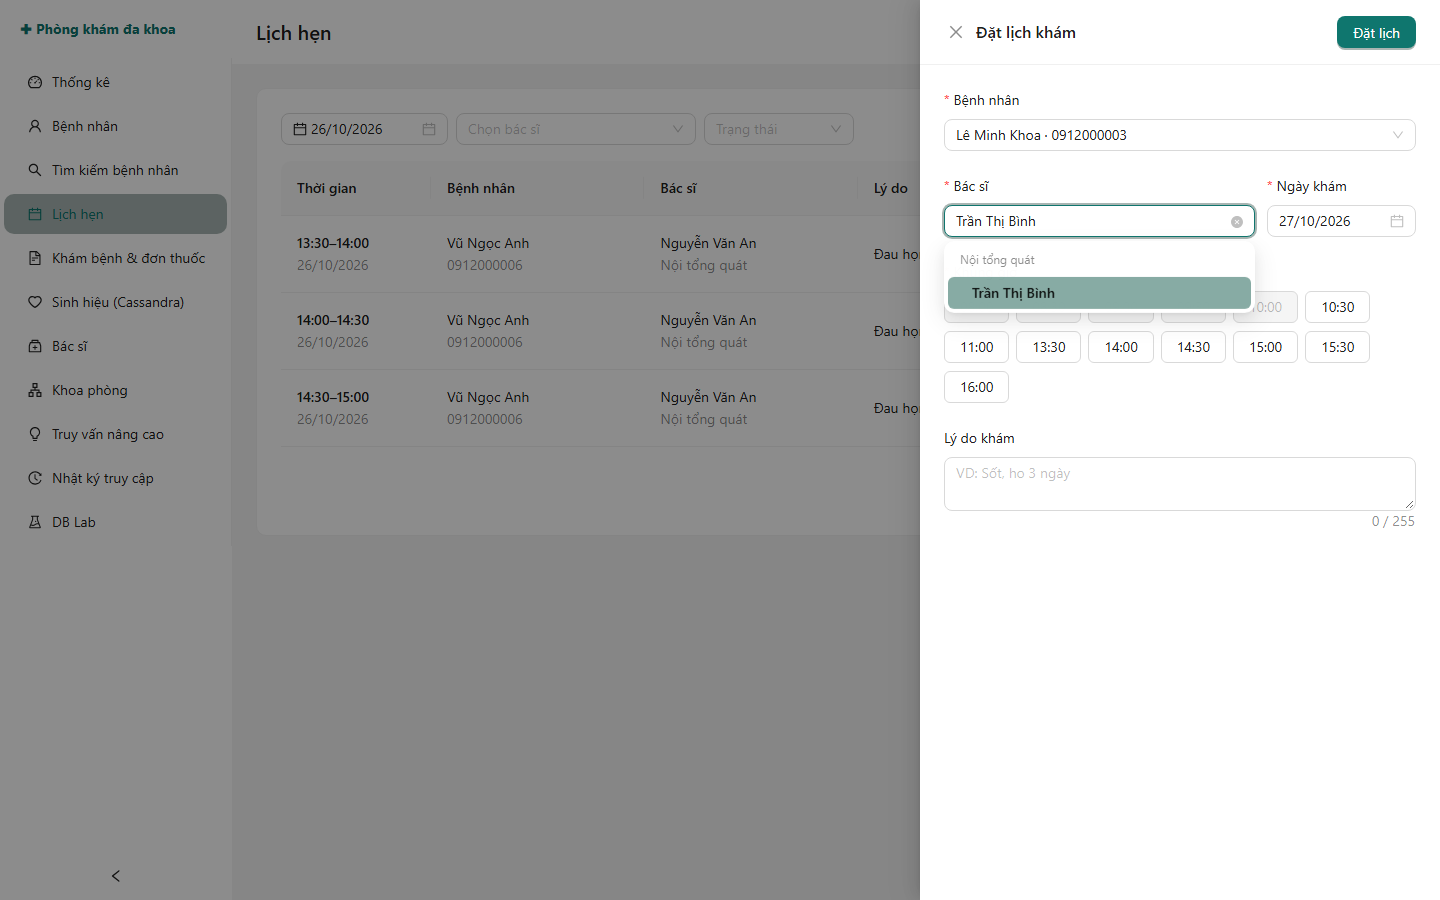
\includegraphics[width=0.95\linewidth]{4-4-fr3-booking.png}
\caption{FR3: đặt lịch với lưới khung giờ trống}
\label{fig:fr3-booking}
\end{figure}

\begin{figure}[H]
\centering
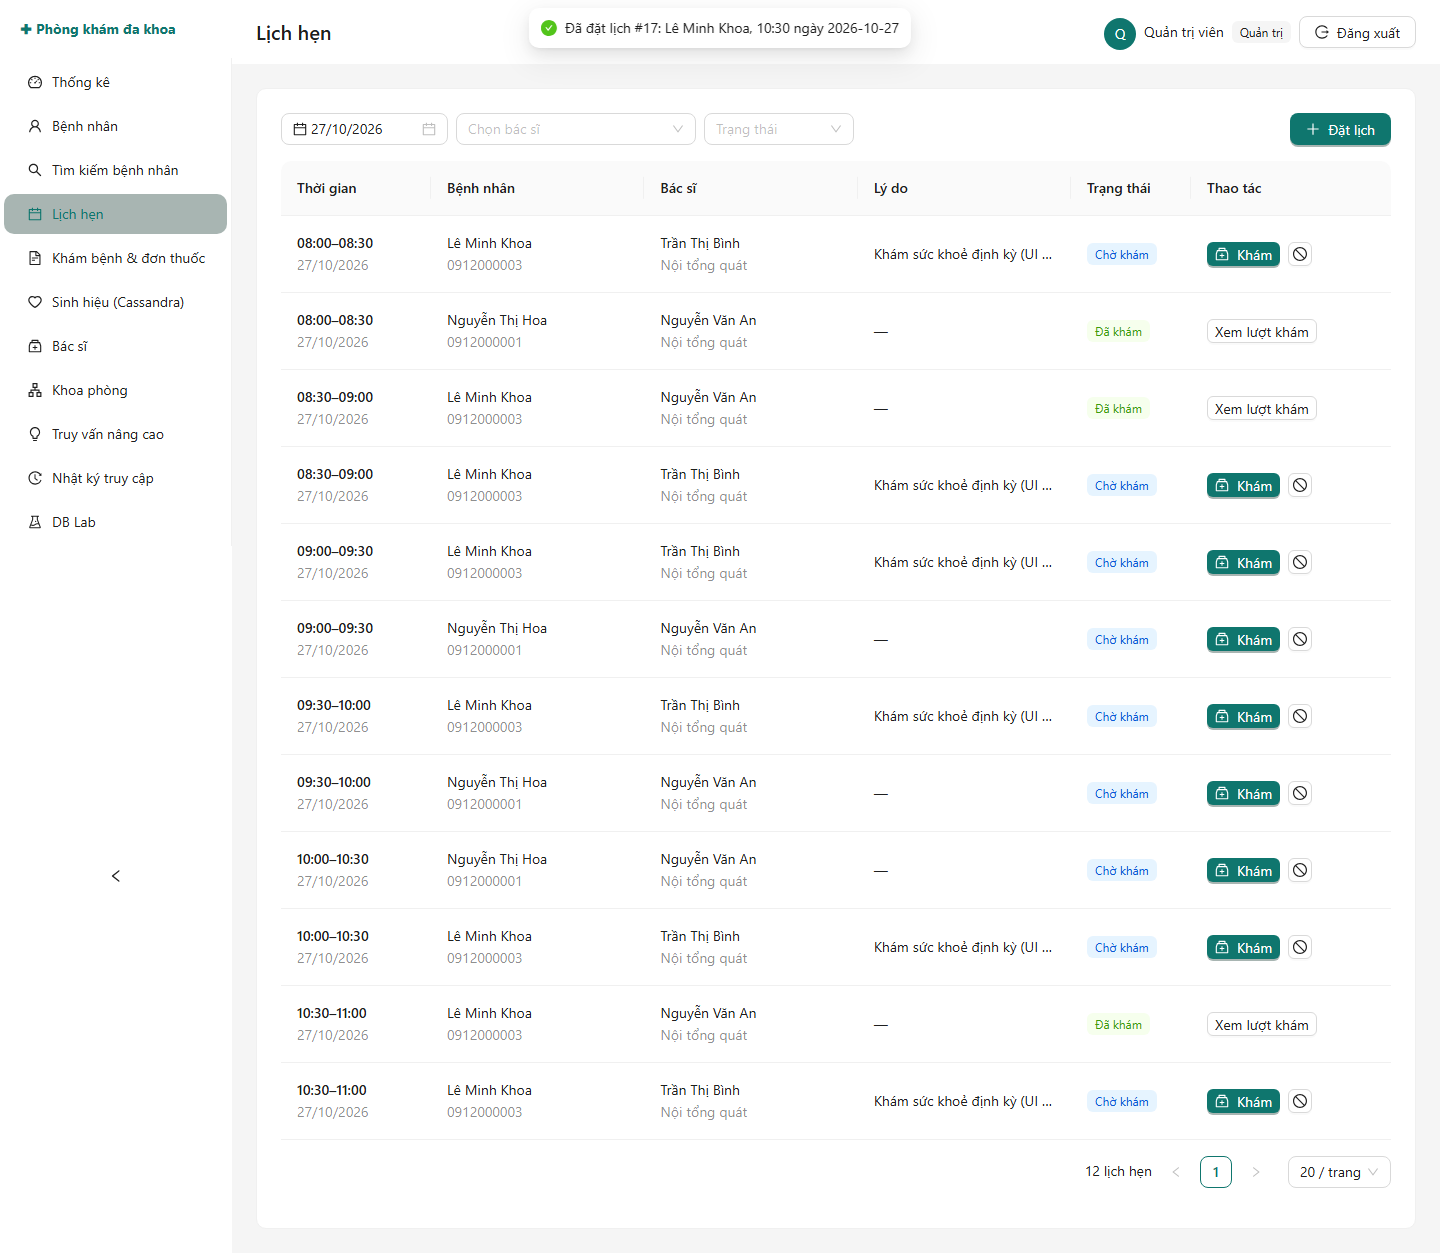
\includegraphics[width=0.95\linewidth]{4-4-fr3-appointments.png}
\caption{FR3: danh sách lịch hẹn}
\label{fig:fr3-list}
\end{figure}

\subsubsection{FR4 và FR6: Khám bệnh và chi tiết lượt khám}
Từ lịch hẹn, bác sĩ bấm \textit{Khám}, form có sẵn bệnh nhân và lý do khám. Bác sĩ nhập chẩn đoán và kê đơn (mỗi thuốc hiện tồn kho), form xem trước hoá đơn (Hình~\ref{fig:fr4}). \texttt{POST /visits} ghi trong \textbf{một transaction}:
\begin{enumerate}
    \item Ghi lượt khám.
    \item Ghi đơn thuốc.
    \item Với mỗi thuốc: \texttt{UPDATE medicines SET stock\_quantity = stock\_quantity - @qty WHERE \ldots{} AND stock\_quantity >= @qty} (kiểm tra và trừ trong một câu, nên không bị lost update), rồi ghi dòng đơn thuốc với giá tại thời điểm kê.
    \item Ghi hoá đơn.
    \item Đóng lịch hẹn.
\end{enumerate}

\begin{lstlisting}[language=SQL, caption={Kiểm tra và trừ tồn kho trong một câu lệnh (\texttt{visits.repository.js})}, label={lst:dispense}]
UPDATE dbo.medicines SET stock_quantity = stock_quantity - @qty
OUTPUT INSERTED.name, INSERTED.unit_price AS unitPrice
WHERE medicine_id = @id AND stock_quantity >= @qty;
\end{lstlisting}

Nếu câu lệnh không cập nhật dòng nào thì thuốc không đủ tồn kho; service ném lỗi 409 và \texttt{withTransaction()} rollback toàn bộ các bước đã ghi trước đó.
Thiếu thuốc ở bất kỳ bước nào thì \textbf{không ghi gì cả}, kèm thông báo nêu tên thuốc. Chi tiết lượt khám lấy bằng \textbf{một câu join 10 bảng} (Hình~\ref{fig:fr6}). Thu ngân bấm \textit{Thanh toán} trên hoá đơn.

\begin{figure}[H]
\centering
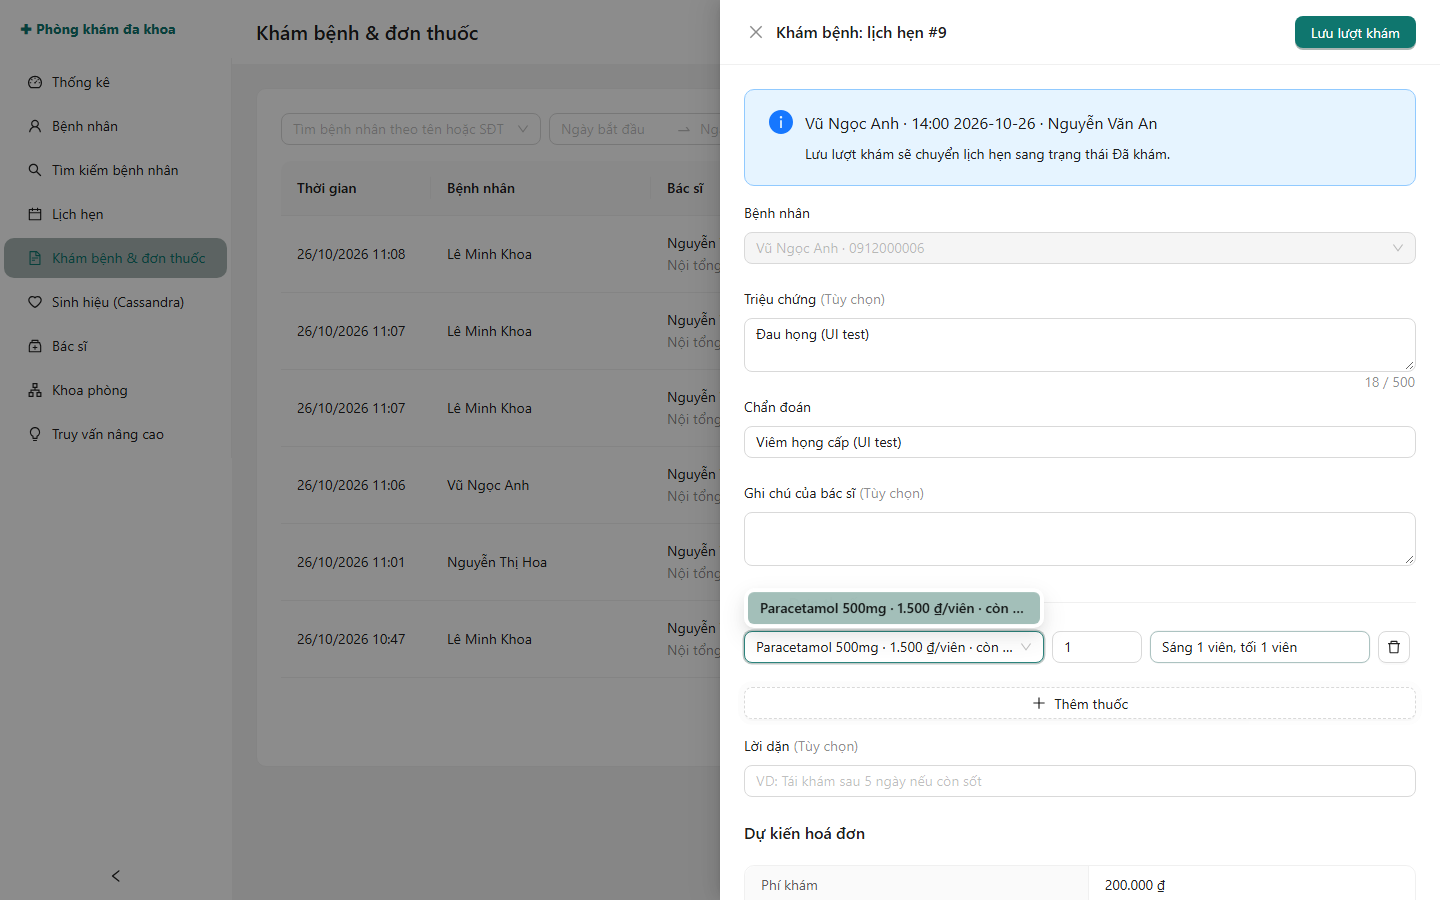
\includegraphics[width=0.95\linewidth]{4-4-fr4-visit-form.png}
\caption{FR4: form khám bệnh và kê đơn}
\label{fig:fr4}
\end{figure}

\begin{figure}[H]
\centering
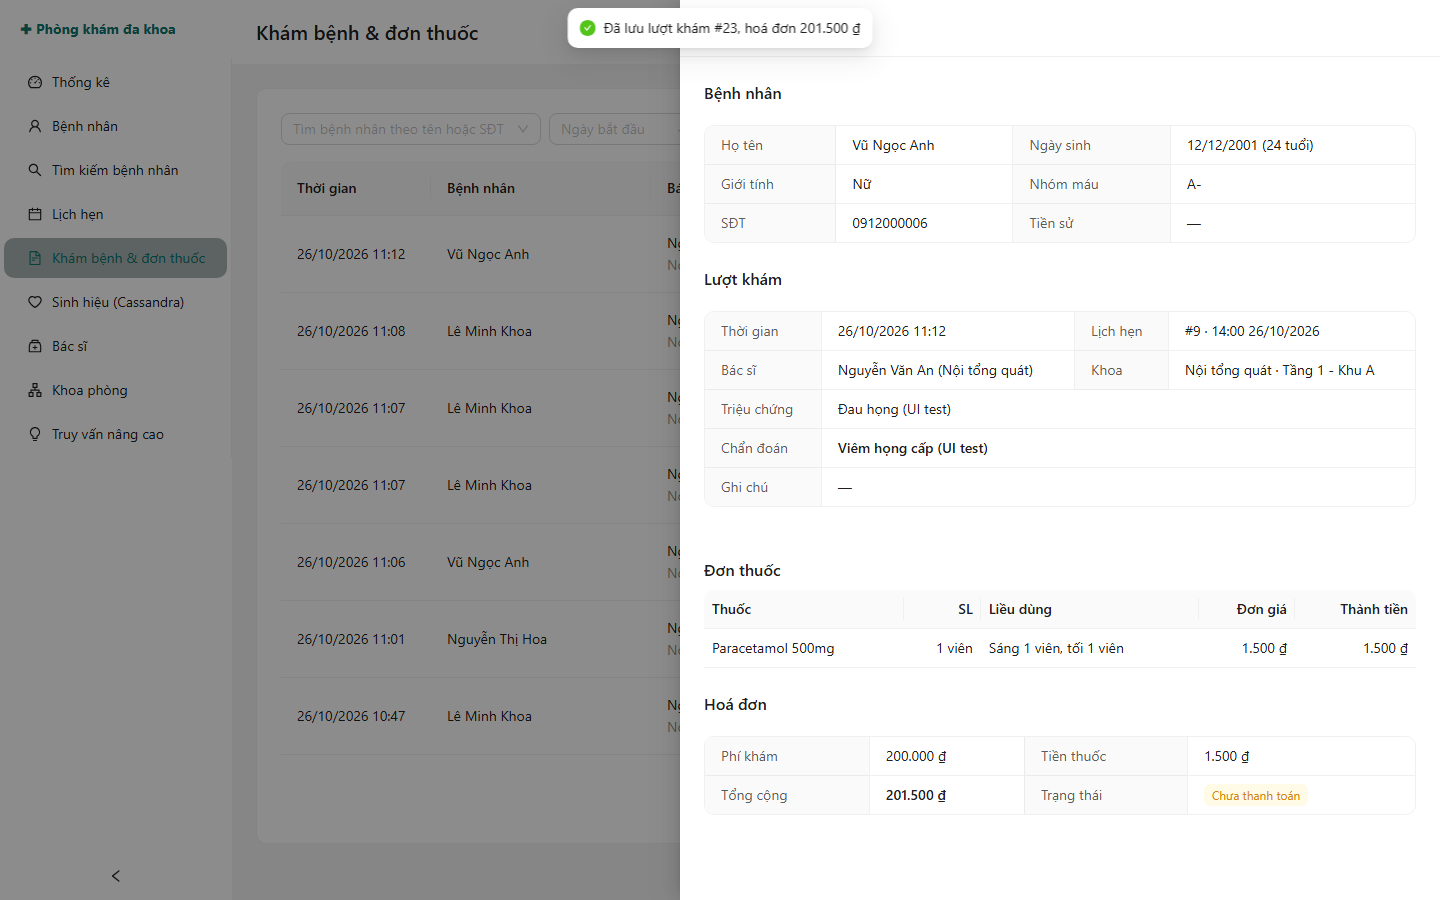
\includegraphics[width=0.95\linewidth]{4-4-fr6-visit-detail.png}
\caption{FR6: chi tiết lượt khám}
\label{fig:fr6}
\end{figure}

\subsubsection{FR9: Theo dõi sinh hiệu}
Thiết bị (trình giả lập trong app) gửi chỉ số. Mỗi lần đo được ghi bằng \textbf{logged batch} vào 3 bảng Cassandra: lịch sử theo (bệnh nhân, ngày), giá trị mới nhất (\texttt{USING TIMESTAMP} = thời điểm đo), cảnh báo theo ngày nếu vượt ngưỡng. Trang theo dõi nhận dữ liệu \textbf{trực tiếp qua Server-Sent Events}, vẽ biểu đồ nhịp tim/SpO$_2$/huyết áp, tô đỏ chỉ số bất thường và liệt kê cảnh báo trong ngày (Hình~\ref{fig:fr9}).

\begin{figure}[H]
\centering
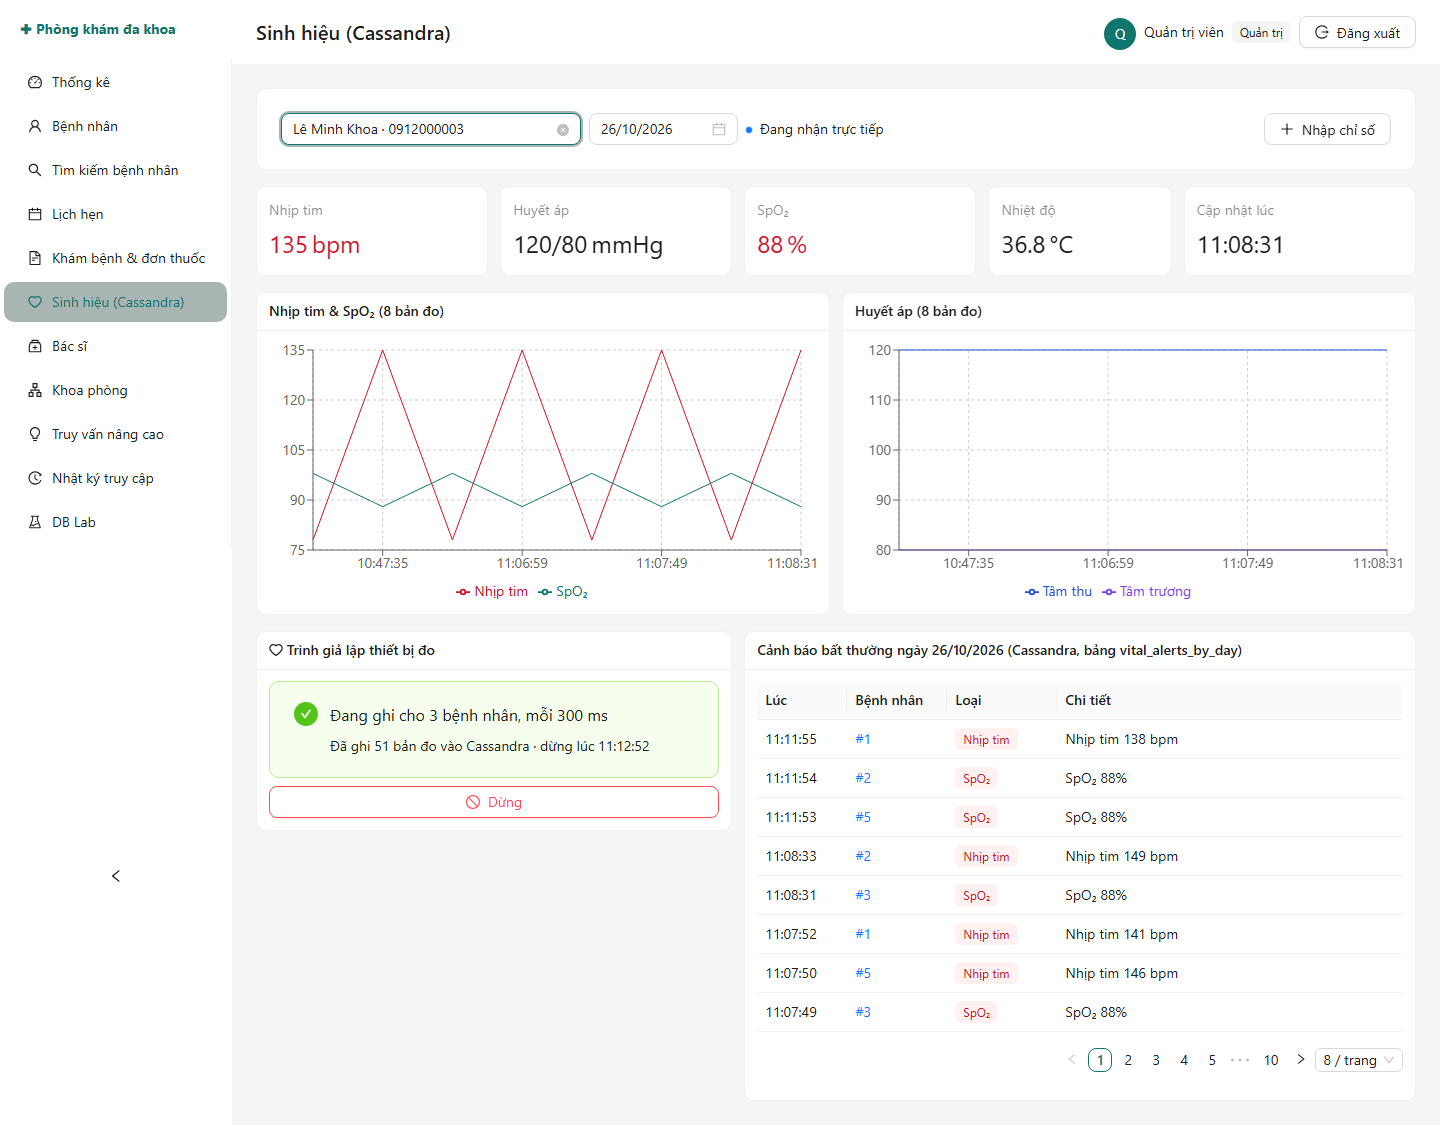
\includegraphics[width=0.95\linewidth]{4-4-fr9-vitals.png}
\caption{FR9: theo dõi sinh hiệu real-time}
\label{fig:fr9}
\end{figure}

\subsubsection{Nhật ký truy cập}
Middleware ghi mỗi request API (bất đồng bộ, không làm chậm request) vào bảng \texttt{access\_logs\_by\_user\_day} (partition theo người dùng + ngày, TTL 90 ngày). Quản trị xem nhật ký theo người dùng và ngày (Hình~\ref{fig:logs}).

\begin{figure}[H]
\centering
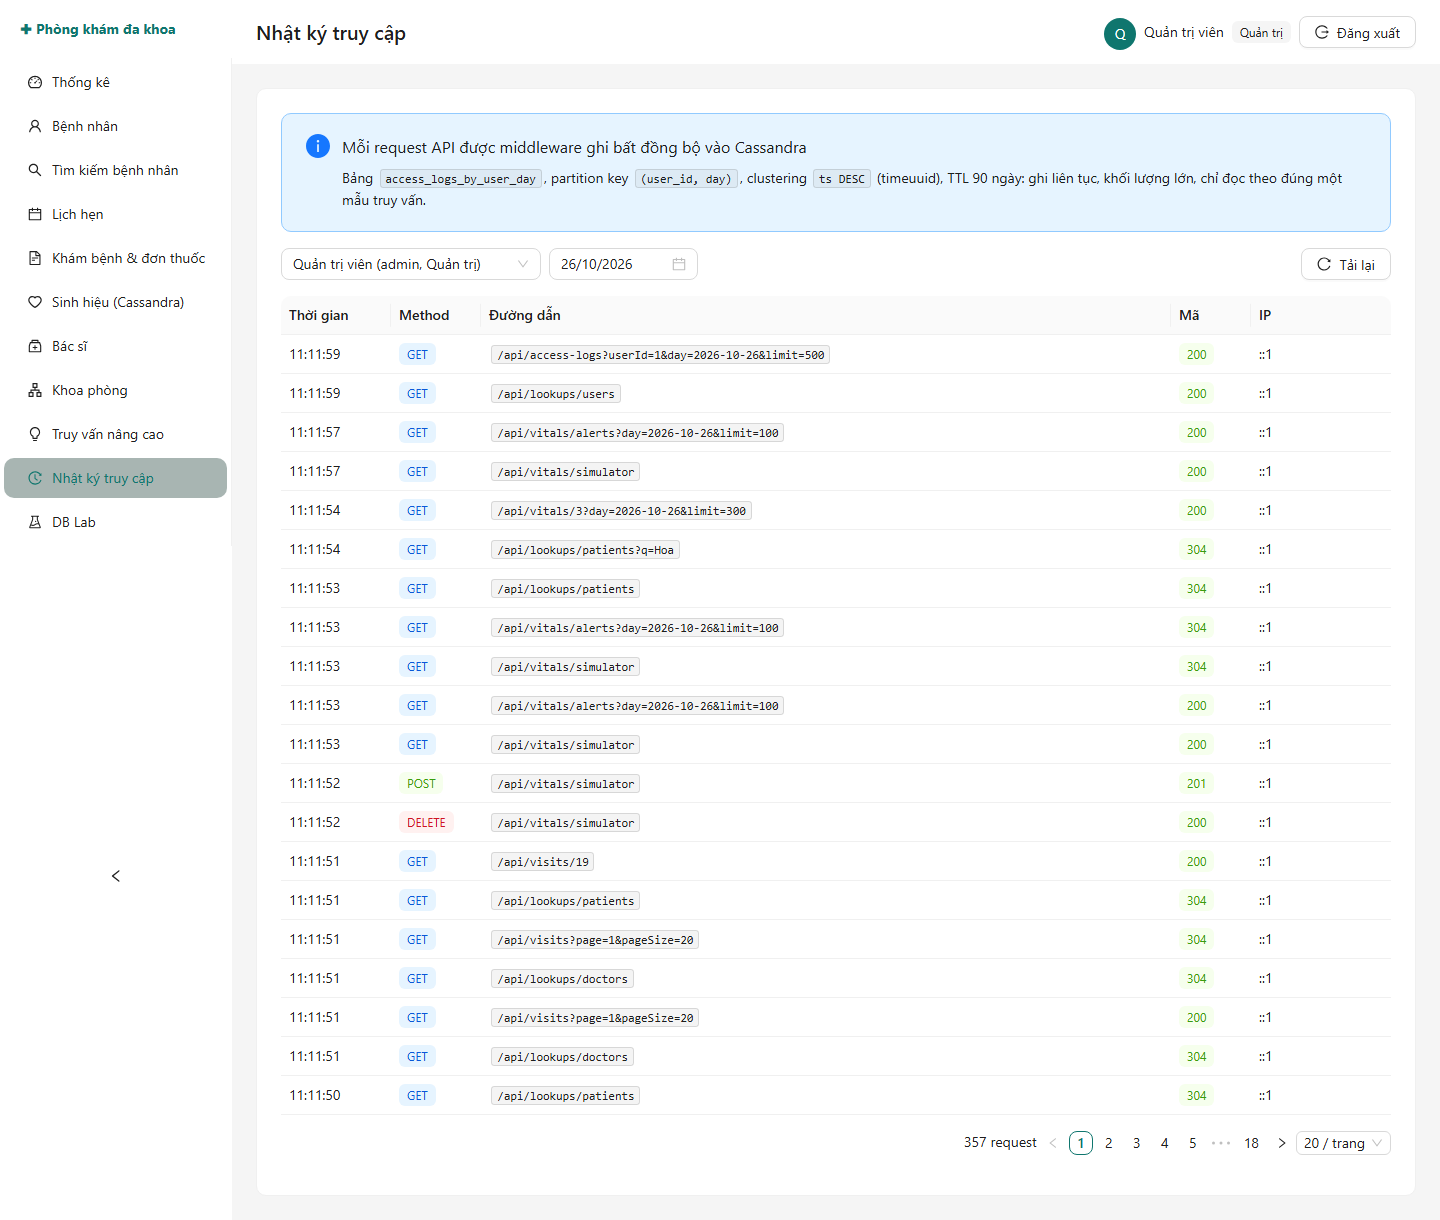
\includegraphics[width=0.95\linewidth]{4-4-access-logs.png}
\caption{Nhật ký truy cập (Cassandra)}
\label{fig:logs}
\end{figure}

\subsubsection{FR1, FR2, FR5, FR7, FR8}
\todo{Dương}{Mô tả hiện thực và ảnh giao diện cho FR1 Bệnh nhân, FR2 Bác sĩ, FR5 Tìm kiếm, FR7 Thống kê, FR8 Truy vấn nâng cao.}

\subsection{Ma trận 8 loại truy vấn}
\label{sec:query-matrix}
\todo{Dương}{Bảng 8 loại a--h (Insert, Delete, Update, Query 1 điều kiện, Query đa điều kiện, Join, Subquery, Aggregate): mỗi loại $\rightarrow$ endpoint, câu SQL/CQL tiêu biểu, chức năng và màn hình tương ứng. Gợi ý nguồn: mục 2 của \texttt{docs/testing/checklist.md}.}

\subsection{DB Lab: đưa nghiên cứu vào ứng dụng}
Trang DB Lab (chỉ ADMIN) chạy các thí nghiệm của Mục~\ref{sec:demo} \textbf{bằng chính code dùng cho script demo} (\texttt{server/src/modules/lab/}), trên một connection pool riêng để thiết lập phiên (isolation, lock timeout) không ảnh hưởng ứng dụng. Mỗi thời điểm chỉ chạy một thí nghiệm.

\begin{table}[H]
\centering
\caption{Các tab của DB Lab}
\label{tab:dblab}
\begin{tabularx}{\linewidth}{|p{3.4cm}|X|}
\hline
\textbf{Tab} & \textbf{Thí nghiệm} \\ \hline
iv. Transaction & Quy trình khám 5 bước, chọn bước gây lỗi; so sánh SQL Server (ROLLBACK, dữ liệu trước = sau) với Cassandra (dở dang / batch) \\ \hline
v. Concurrency & Ma trận hiện tượng $\times$ mức cô lập; đặt trùng lịch $N$ request theo 5 cách; tạo deadlock và xem khoá \\ \hline
vi. Backup \& recovery & Backup full/diff/log, lịch sử msdb; point-in-time restore sau sự cố ``UPDATE quên WHERE'' \\ \hline
i--iii & \colorbox{yellow!40}{TODO (Dương): lưu trữ, chỉ mục, kế hoạch thực thi} \\ \hline
\end{tabularx}
\end{table}

\begin{figure}[H]
\centering
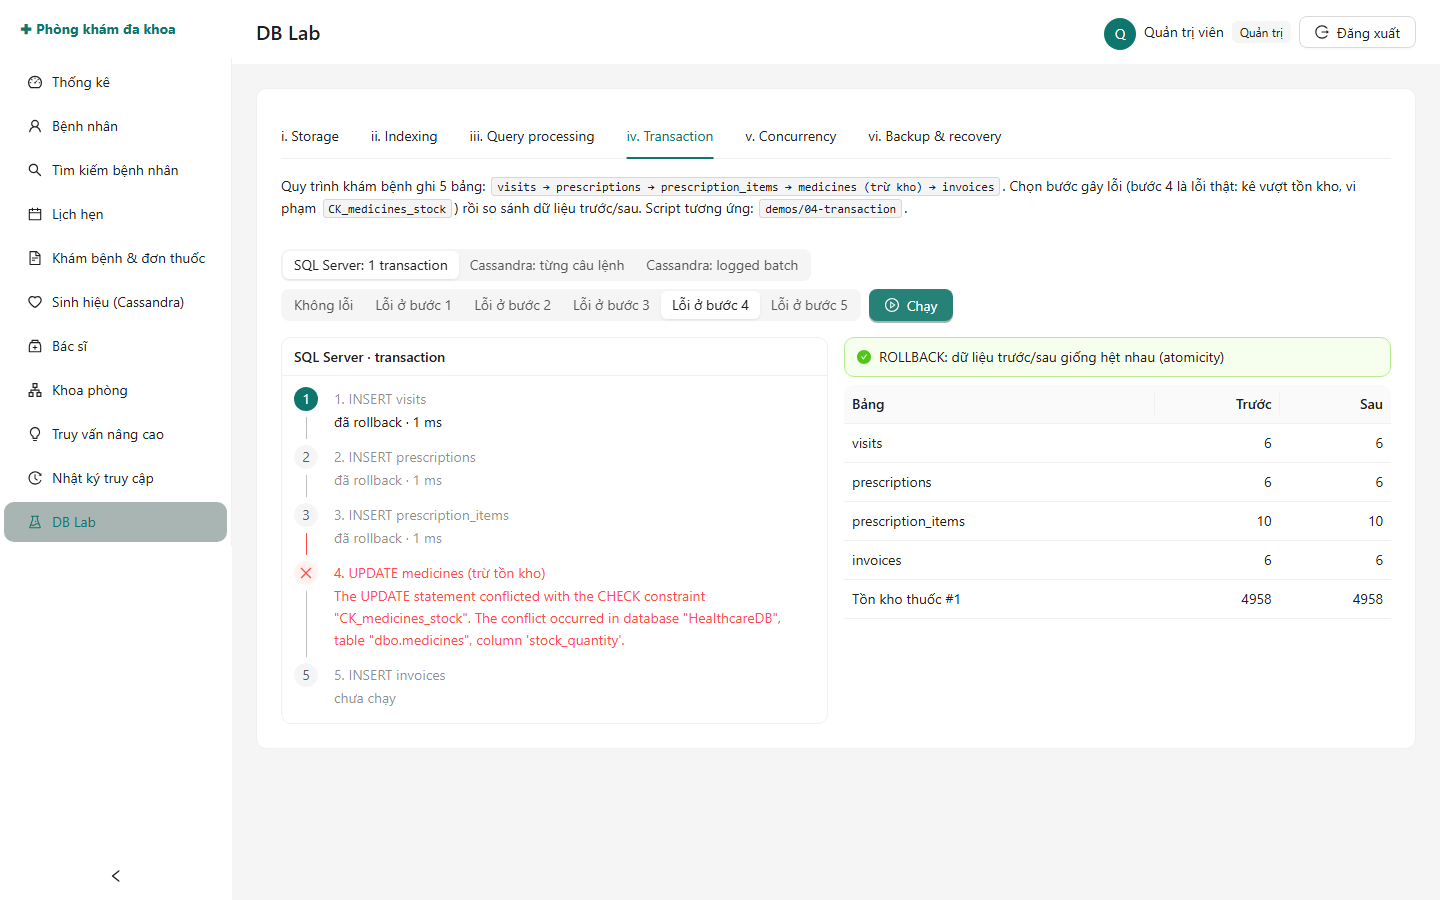
\includegraphics[width=0.95\linewidth]{4-6-lab-transaction.png}
\caption{DB Lab: tab Transaction}
\label{fig:lab-tx}
\end{figure}

\begin{figure}[H]
\centering
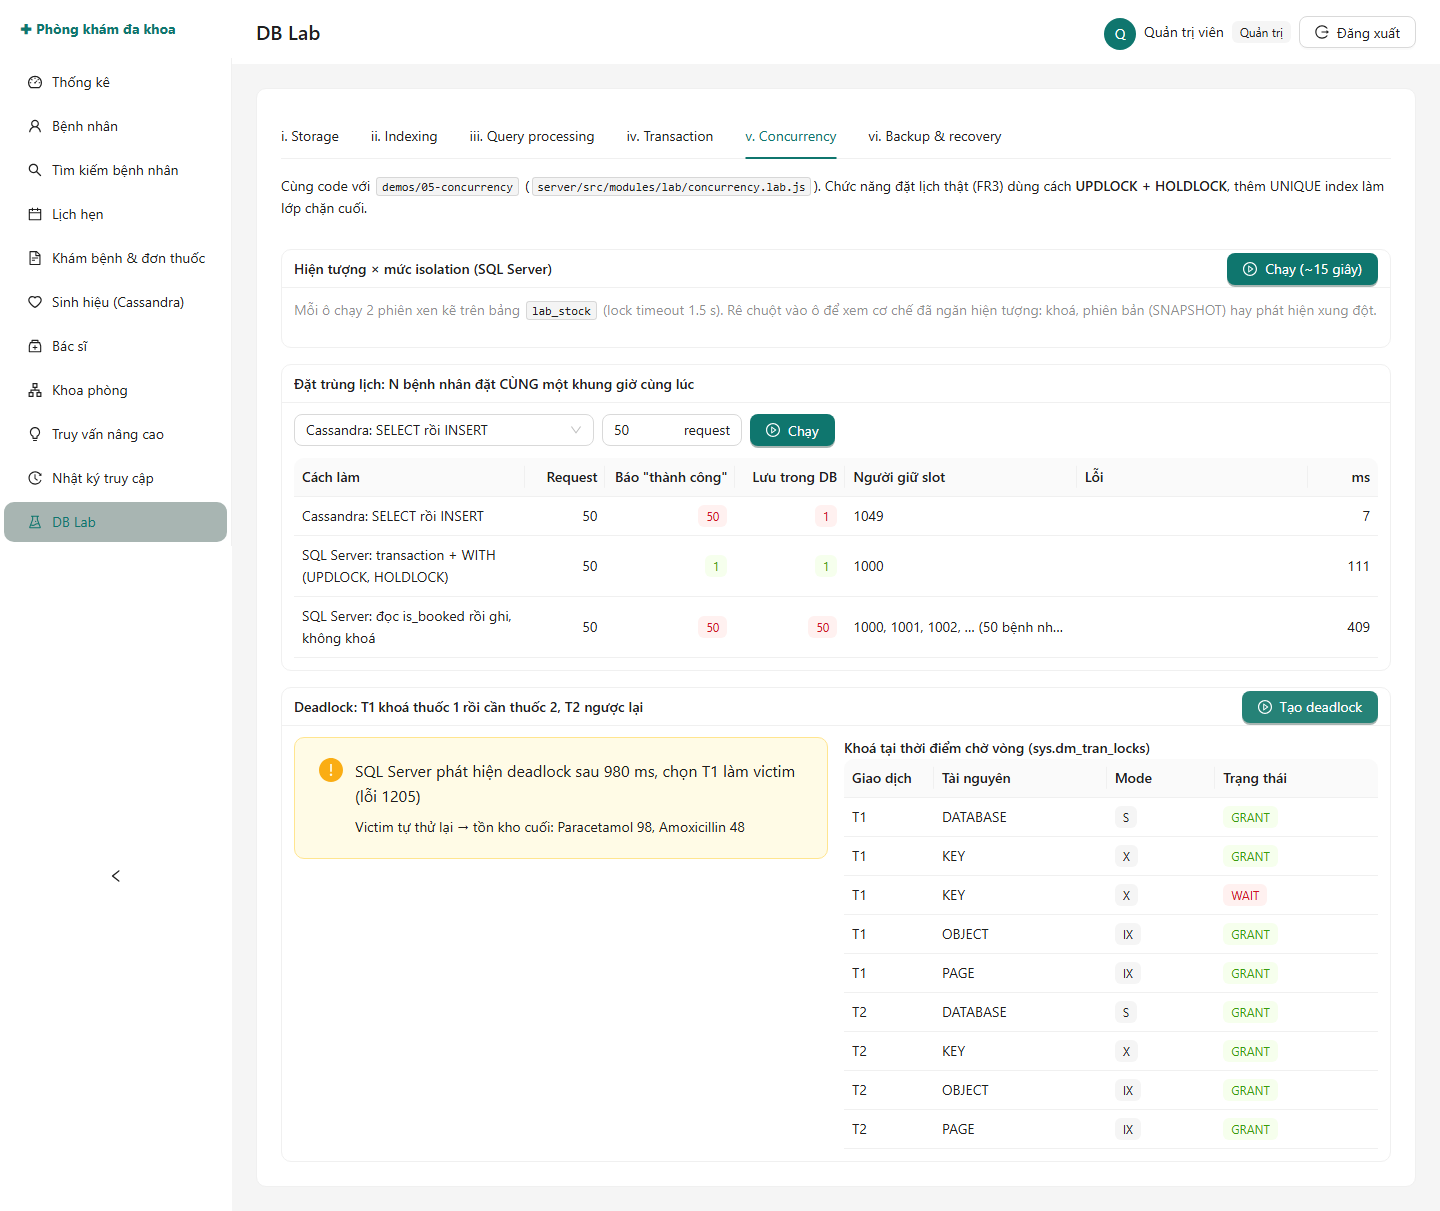
\includegraphics[width=0.95\linewidth]{4-6-lab-concurrency.png}
\caption{DB Lab: tab Concurrency}
\label{fig:lab-cc}
\end{figure}

\begin{figure}[H]
\centering
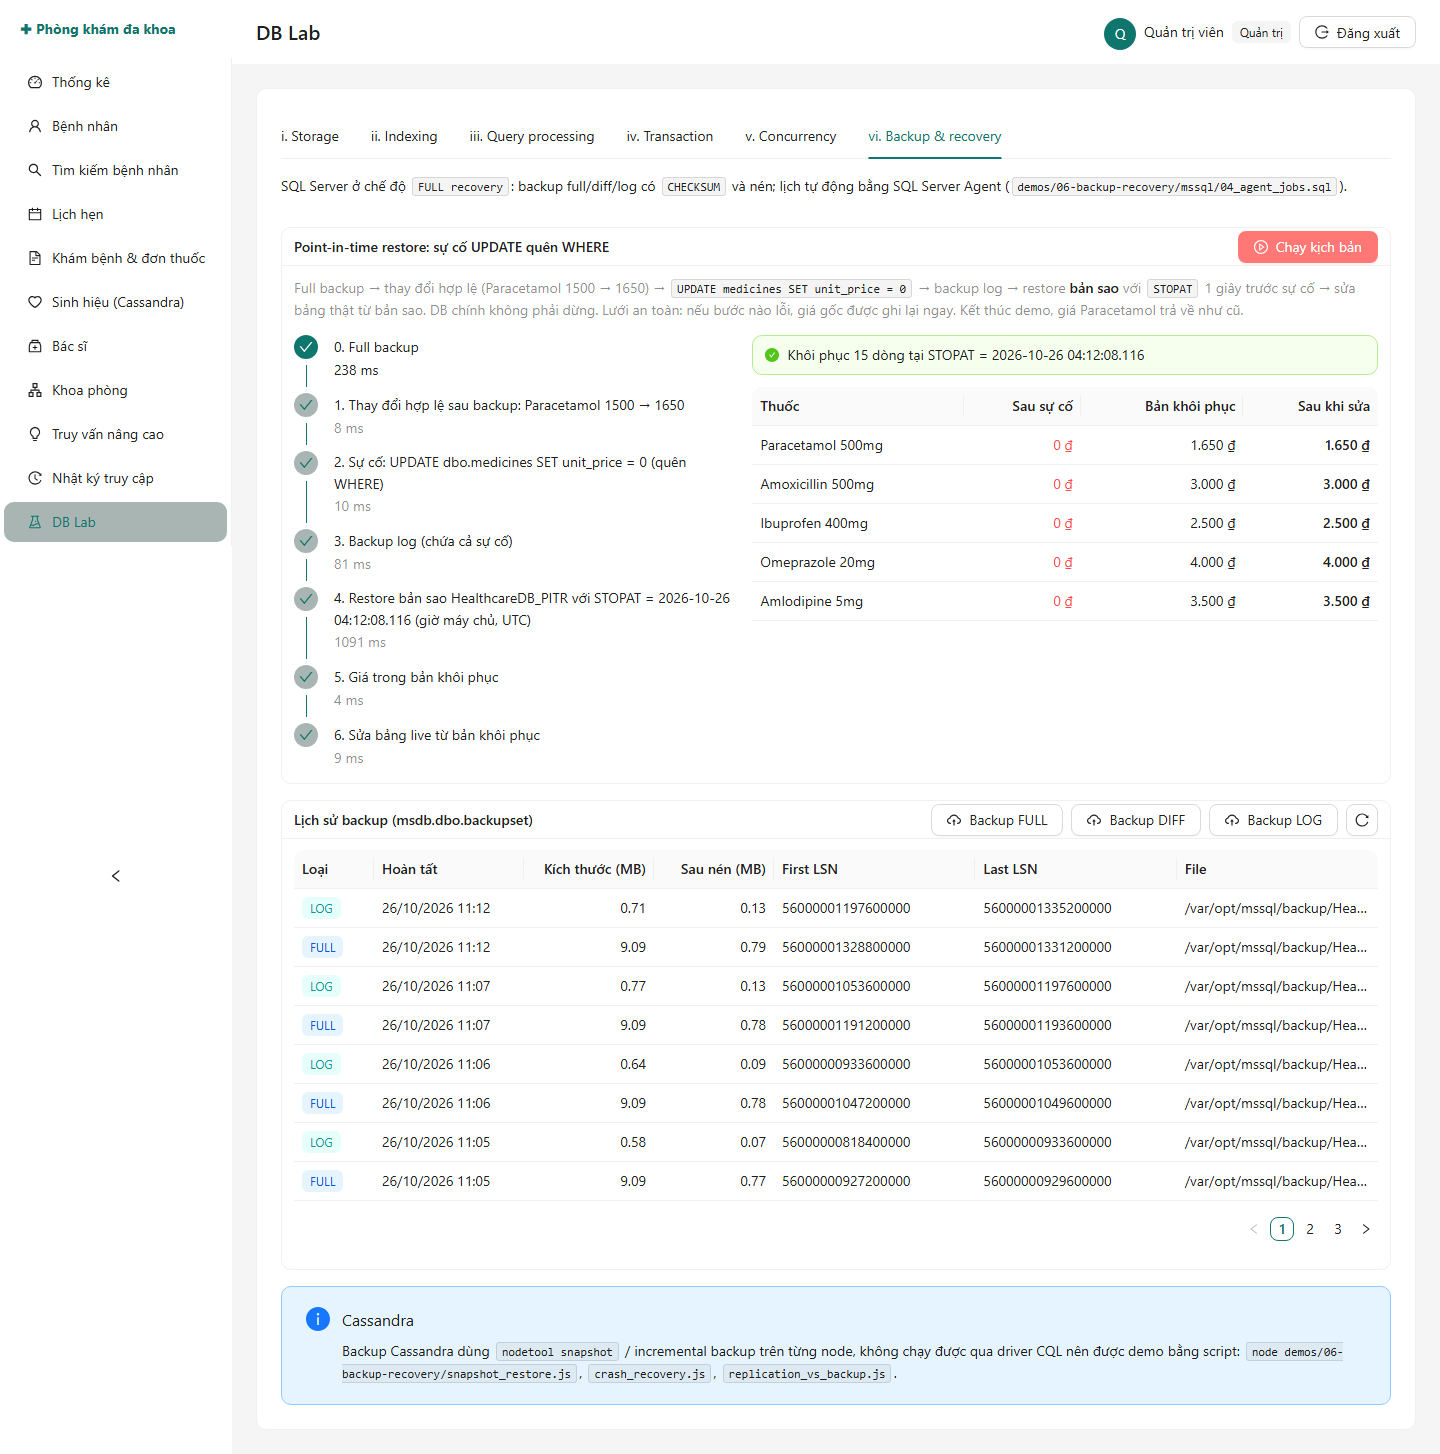
\includegraphics[width=0.95\linewidth]{4-6-lab-backup.png}
\caption{DB Lab: tab Backup \& recovery}
\label{fig:lab-backup}
\end{figure}

\subsection{Kiểm thử}
Ứng dụng được kiểm thử ở hai mức:
\begin{itemize}
    \item \textbf{Test API end-to-end} (\texttt{server/test/hoang-features.e2e.test.js}, chạy bằng \texttt{npm run test:e2e -w server}): 14 test gọi API thật trên hai DB đang chạy. Kết quả: \textbf{14/14 đạt}.
    \item \textbf{Kiểm thử giao diện} bằng trình duyệt headless (Playwright) trên 9 luồng nghiệp vụ: \textbf{0 lỗi console}.
    \item \textbf{Test chéo thủ công} theo checklist 24 ca (\texttt{docs/testing/checklist.md}): mỗi thành viên kiểm thử chức năng của người kia.
\end{itemize}

\begin{table}[H]
\centering
\caption{Các ca kiểm thử API tiêu biểu}
\label{tab:e2e}
\begin{tabularx}{\linewidth}{|p{3cm}|X|X|}
\hline
\textbf{Chức năng} & \textbf{Ca kiểm thử} & \textbf{Kết quả mong đợi} \\ \hline
FR3 Đặt lịch & 20 request đặt \textbf{cùng một} khung giờ gửi đồng thời & Đúng 1 thành công (201), 19 nhận 409 \\ \hline
FR3 Đặt lịch & Đặt lại khung giờ đã có lịch; xoá lịch đang chờ; huỷ rồi xoá & 409; 409; khung giờ mở lại, xoá được (204) \\ \hline
FR3 Đặt lịch & Đặt khung giờ đã qua; dữ liệu sai kiểu & 400 kèm chi tiết lỗi \\ \hline
FR4 Khám bệnh & Kê đơn hợp lệ 2 thuốc từ lịch hẹn & Hoá đơn = phí khám + tiền thuốc; tồn kho giảm đúng; lịch hẹn \textit{Đã khám} \\ \hline
FR4 Khám bệnh & Kê Salbutamol vượt tồn kho & 409 nêu tên thuốc; tồn kho và số lượt khám \textbf{không đổi} \\ \hline
FR6 Chi tiết & Lấy chi tiết lượt khám vừa tạo, thanh toán 2 lần & Đủ bệnh nhân, khoa, hoá đơn; lần thanh toán thứ 2 nhận 409 \\ \hline
FR9 Sinh hiệu & Ghi nhịp tim 135, SpO$_2$ 88; mở luồng SSE & Sinh 2 cảnh báo; luồng SSE đẩy bản đo mới \\ \hline
Nhật ký & Gọi API bằng một tài khoản & Mọi request được ghi, token bị che \\ \hline
Phân quyền & Bác sĩ đặt lịch; bác sĩ gọi API DB Lab & 403 \\ \hline
\end{tabularx}
\end{table}

Các lỗi phát hiện trong quá trình kiểm thử và đã sửa: luồng SSE bị proxy của Vite giữ header nên trang sinh hiệu không nhận dữ liệu; phí khám dự kiến hiển thị bằng 0 với tài khoản bác sĩ; Vite 8 bị crash native khi hot reload nên hạ về Vite 7.
